\section{Моделирование динамических процессов в ледовом острове}

\subsection{Геологическая модель}

Рассмотрим в двумерном случае ледовый остров шириной 300 м. и высотой 10 м., покоящийся на дне моря глубиной 8 м.

\begin{figure}[htb]
    \centering
    \includegraphics[trim={0.5cm 3.5cm 0.5cm 2.0cm},clip,width=0.75\textwidth]{images/gas_field/gas_field_scheme.png}
    \caption{Схема геологической модели.}
    \label{fig:island}
\end{figure}

Грунт под островом будем считать состоящим из придонного слоя глубиной 10 м. и слоя осадочных пород глубиной 600 м. В некоторых случаях мы будем также рассматривать  газоносный слой. Бур будем считать расположенным посередине длины острова на глубине 20 м.

Параметры рассматриваемых сред приведены в таблице \autoref{tab:geo}.

\renewcommand{\arraystretch}{1.2}
\begin{table}[htb]
\centering
    \begin{tabular}{|l|c|c|c|}
    \hline
    Среда & $c_p$, м/с & $c_s$, м/с & $\rho$, кг/м\textsuperscript{3} \\ \hline
    Лёд & 3940 & 2493 & 917 \\ \hline
    Вода & 1500  & --- & 1025 \\ \hline
    Придонный грунт & 1806 & 316 & 2000 \\ \hline
    Осадочные породы & 2250 & 1000 & 2000 \\ \hline
    \end{tabular}
\caption{Параметры рассматриваемых сред.}
\label{tab:geo}
\end{table}
\renewcommand{\arraystretch}{1.0}

\subsection{Математическая модель среды}

\subsubsection{Уравнения}

Рассматриваемые среды (см. таблицу \autoref{tab:geo}) будем считать сплошными, однородными, изотропными и несжимаемыми. В описанной постановке присутствуют как жидкие среды (вода, окружающая остров), так и твёрдые среды (лёд и слои грунта).

Жидкие среды в двумерном случае в декартовой эйлеровой системе координат описываются акустическим волновым уравнением

\begin{equation}
    \begin{dcases}
        \rho \frac{\partial \vec{v}(x,y,t)}{\partial t} = -\nabla p (x,y,t) \\
        \frac{\partial p(x,y,t)}{\partial t} = -\rho c^2 \Div \vec{v}(x,y,t)
    \end{dcases}
    \label{eq:acoustic_wave_eq}
\end{equation}

где $\rho$ --- плотность среды, $\vec{v}(x,y,t)$ --- вектор скорости (производная вектора смещения частицы среды $\vec{u}(x,y,t)$ по времени), $p(x,y,t)$ --- давление, $c$ --- скорость звука в жидкости.

Твёрдые среды в двумерном случае в декартовой эйлеровой системе координат описываются уже  упругим волновым уравнением
\begin{equation}
    \begin{dcases}
        \rho \frac{\partial \vec{v}(x,y,t)}{\partial t} = \Div^T \pmb{\sigma} (x,y,t) \\
        \frac{\partial \pmb{\sigma}(x,y,t)}{\partial t} = \rho \left(c_p^2 - 2c_s^2\right) \Div \vec{v}(x,y,t) \pmb{I} + \rho c_s^2 \left(\nabla \otimes \vec{v}(x,y,t) + \left[ \nabla \otimes \vec{v}(x,y,t)\right]^T \right)
    \end{dcases}
    \label{eq:elastic_wave_eq}
\end{equation}

где $\pmb{\sigma}(x,y,t)$ --- симметричный тензор напряжений Коши второго ранга, $c_p$ и $c_s$ --- скорости продольной и поперечной волн соответственно, $\pmb{I}$ --- единичный тензор второго ранга, операция $\otimes$ --- тензорное произведение векторов.

Далее для краткости мы будем опускать значок у вектора скорости, то есть будем писать $v$, подразумевая при этом вектор $\vec{v}$. Также мы будем опускать параметры $(x,y,t)$ у зависящих от них величин.

\subsubsection{Контактные условия}

Между средами необходимо поставить контактные условия, которые изображены на \autoref{fig:contacts}.

\begin{figure}[H]
    \centering
    \includegraphics[trim={90pt 35pt 90pt 60pt},clip,width=0.75\textwidth]
    {images/gas_field/contacts.png}
    \caption{Схема контактных условия: 1 --- контактное условие полного слипания, 2 --- контактное условие между упругой и акустической средами, 3 --- контактное условие скольжения, 4 --- контактное условие отражения.}
    \label{fig:contacts}
\end{figure}

Здесь и далее мы будем обозначать контактирующие среды (или расчётные сетки) индексами $L$ и $R$ --- левая и правая среды соответственно. Вектор внешней нормали к левой под-области обозначим как $n$.

\begin{enumerate}
    \item Контактное условие полного слипания ставится между слоями твёрдых сред. Физически оно означает возможность беспрепятственного распространения упругих волн. Для этого требуется равенство скоростей и векторов нормального напряжения на границе раздела.
    
    Математически условие полного слипания записывается следующим образом
    \begin{equation}
    \begin{dcases}
        v_L = v_R \\
        \pmb{\sigma}_L \cdot n = \pmb{\sigma}_R \cdot n
    \end{dcases}
    \end{equation}
    
    \item Контактное условие между упругой и акустической средой используется для реализации перехода волн из твёрдых сред в жидкость и обратно. Оно отличается от условий полного слипания, т.к. в данном случае контактирующие среды описываются разными уравнениями (см. \eqref{eq:acoustic_wave_eq} и  \eqref{eq:elastic_wave_eq}).
    
    Если считать, что акустическая среда отвечает индексу $L$, а упругая --- $R$, то данное условие запишется как
    \begin{equation}
    \begin{dcases}
        v_L \cdot n = v_R \cdot n \\
        \pmb{\sigma} \cdot n + p n = 0
    \end{dcases}
    \end{equation}
    
    Физически это условие означает не-протекание жидкости в твёрдое тело, и наоборот. Для этого требуется равенство нормальных скоростей. первое уравнение, и равенство нормального вектора напряжений на контактной границе, второе уравнение.
    
    \item Контактное условие свободного скольжения ставится между ледовым островом и грунтом. В отличие от случая контакта двух слоёв грунта, когда применяется условие полного слипания, лёд и придонный слой могут двигаться друг относительно друга. Это явление известно на практике, так, например, наблюдается "соскальзывание" ледников с поверхностей гор. Таким образом требуется использование специального контактного условия.
    \begin{equation}
    \begin{dcases}
        v_L \cdot n = v_R \cdot n \\
        n \cdot \pmb{\sigma}_L \cdot n = n \cdot \pmb{\sigma}_L \cdot n \\
        n \cdot \sigma_{L/R} \cdot n = \sigma_{L/R} \cdot n
    \end{dcases}
    \end{equation}

    \item Контактное условие полного отражения (свободной границы) ставится на границе раздела осадочных пород и газоносного слоя. Применение такого условия не является вполне физически верным, однако для нашей задачи его применение вполне оправдано.

    \begin{equation}
        \pmb{\sigma} \cdot n = 0
    \end{equation}

\end{enumerate}

\subsubsection{Граничные условия}

Граничные условия расчётной области изображены на \autoref{fig:borders}.

\begin{figure}[htb]
    \centering
    \includegraphics[trim={90pt 35pt 90pt 60pt},clip,width=0.75\textwidth]
    {images/gas_field/border_conds.png}
    \caption{Схема граничных условий: a --- граничное условие поглощения, b --- граничное условие нулевого давления.}
    \label{fig:borders}
\end{figure}

\begin{enumerate}
    \item Поглощающие (не-отражающие) граничные условия используются при рассмотрении ограниченной под-области бесконечного физического региона. В данном случае водяной, придонный, газоносный слои и слой осадочных пород продолжаются за границы расчётной области налево, направо и, для газоносного слоя, вниз. Поэтому на их краях необходимо использовать поглощающие граничные условия. \footnote{Поглощающие условия будут рассмотрены подробнее в главе \ref{sec:absorbing}.}
    
    Для упругих сред это условие запишется в виде
    
    \begin{equation}
    \begin{dcases}
        v_{l-2}^n = 
        v_{l-1}^n = 
        v_{l}^n \\
        \pmb{\sigma}_{l-2}^n = 
        \pmb{\sigma}_{l-1}^n = 
        \pmb{\sigma}_{l}^n
    \end{dcases}
    \end{equation}
    
    А для акустических сред в виде
    
    \begin{equation}
    \begin{dcases}
        v_{l-2}^n = 
        v_{l-1}^n = 
        v_{l}^n \\
        p_{l-2}^n = 
        p_{l-1}^n = 
        p_{l}^n
    \end{dcases}
    \end{equation}
    
    здесь верхний индекс $n$ обозначает момент времени $t_n$, а нижний --- номер сеточного узла, при этом узел $l$ является граничным, а узлы $l-1$ и $l-2$ --- его соседями по одной из осей. Такая форма записи будет верна для левой, правой и нижней границе при соответствующем выборе значений координатных индексов.
    
    \item Граничное условие нулевого давления применяется на границе сред с воздухом. В нашей задаче мы не учитываем влияние атмосферного давления на исследуемые процессы, считая его пренебрежимо малым. Следовательно мы принимаем $p=0$ на границах вода-воздух и лёд-воздух.
\end{enumerate}

\subsection{Численный метод}

\subsubsection{Сеточно-характеристический метод}

Для решения систем уравнений в частных производных \eqref{eq:elastic_wave_eq} и \eqref{eq:acoustic_wave_eq} воспользуемся сеточно-характеристическим методом на регулярных прямоугольных сетках. Получим его для системы \eqref{eq:acoustic_wave_eq}, описывающей упругие среды. Для системы \eqref{eq:acoustic_wave_eq} он получается абсолютно аналогично если учесть, что для акустических сред $\sigma_{xx} = \sigma_{yy} = p$ и $\sigma_{xy}=0$.

Будем работать в декартовой прямоугольной системе координат. Введём обозначение 
\begin{equation}
    \varphi = \begin{pmatrix} v_x \\ v_y \\ \sigma_{xx} \\ \sigma_{xy} \\ \sigma_{yy} \end{pmatrix}
\end{equation}

Нижние индексы здесь обозначают соответствующие компоненты ветора скорости $v$ и тензора напряжений $\pmb{\sigma}$.

Запишем гиперболическую полную систему линейный дифференциальных уравнений в частных производных \eqref{eq:elastic_wave_eq} в канонической матричной форме

\begin{equation}
    \dfrac{\partial \varphi}{\partial t} + 
    \pmb{A} \dfrac{\partial \varphi}{\partial x} + 
    \pmb{B} \dfrac{\partial \varphi}{\partial y} = 0
\end{equation}

\begin{equation}
    \pmb{A} = \begin{pmatrix}
        0 & 0 & -\frac{1}{\rho} & 0 & 0 \\
        0 & 0 & 0 & -\frac{1}{\rho} & 0 \\
        -(\lambda+2\mu) & 0 & 0 & 0 & 0 \\
        0 & -\mu & 0 & 0 & 0 \\
        -\lambda & 0 & 0 & 0 & 0
    \end{pmatrix}
\end{equation}

\begin{equation}
    \pmb{B} = \begin{pmatrix}
        0 & 0 & 0 & 0 & 0 \\
        0 & 0 & -\frac{1}{\rho} & 0 & 0 \\
        0 & -\lambda & 0 & 0 & 0 \\
        -\mu & 0 & 0 & 0 & 0 \\
        0 & -(\lambda+2\mu) & 0 & 0 & 0
    \end{pmatrix}
\end{equation}

Здесь $\lambda$ и $\mu$ --- параметры Ламе, которые выражаются через заданные для конкретных сред скорости продольных и поперечных волн

\begin{equation}
    \begin{dcases}
        c_p = \sqrt{\dfrac{\lambda + 2\mu}{\rho}} \\
        c_s = \sqrt{\dfrac{\mu}{\rho}}
    \end{dcases}
\end{equation}

\begin{equation}
    \begin{dcases}
        \lambda = \left(c_p^2 - 2 c_s^2\right) \rho \\
        \mu = c_s^2 \rho
    \end{dcases}
\end{equation}

Используя метод расщепления для системы, записанной в каноническом виде, получим систему

\begin{equation}
    \begin{dcases}
        \dfrac{\partial \varphi_x}{\partial t} + \pmb{A} \dfrac{\partial \varphi_x}{\partial x} = 0 \\
        \dfrac{\partial \varphi_y}{\partial t} + \pmb{B} \dfrac{\partial \varphi_y}{\partial y} = 0
    \end{dcases}
    \label{eq:rashepl_elastic}
\end{equation}

Заметим, что матрицы $\pmb{A}$ и $\pmb{B}$ можно диагонализовать
%https://www.wolframalpha.com/input/?i=%7B%7B0%2C0%2C-1%2Fp%2C0%2C0%7D%2C%7B0%2C0%2C0%2C-1%2Fp%2C0%7D%2C%7B-%28l%2B2m%29%2C0%2C0%2C0%2C0%7D%2C%7B0%2C-m%2C0%2C0%2C0%7D%2C%7B-l%2C0%2C0%2C0%2C0%7D%7D
%https://www.wolframalpha.com/input/?i=%7B%7B0%2C0%2C0%2C-1%2Fp%2C0%7D%2C%7B0%2C0%2C0%2C0%2C-1%2Fp%7D%2C%7B0%2C-l%2C0%2C0%2C0%7D%2C%7B-m%2C0%2C0%2C0%2C0%7D%2C%7B0%2C-%28l%2B2m%29%2C0%2C0%2C0%7D%7D

\begin{gather*}
    \pmb{A} = \pmb{S}^{-1}_1 \pmb{\Lambda}_1 \pmb{S}_1 \\
    \pmb{B} = \pmb{S}^{-1}_2 \pmb{\Lambda}_2 \pmb{S}_2
\end{gather*}
\begin{gather*}
    \pmb{S}^{-1}_1 = 
    \begin{pmatrix}
        0 & 0 & 0 & \sqrt{\frac{\lambda + 2\mu}{\lambda^2 \rho}} & -\sqrt{\frac{\lambda + 2\mu}{\lambda^2 \rho}} \\
        0 & \frac{1}{\sqrt{\mu\rho}} & -\frac{1}{\sqrt{\mu\rho}} & 0 & 0 \\
        0 & 0 & 0 & \frac{2\mu}{\lambda} + 1 & \frac{2\mu}{\lambda} + 1 \\
        0 & 1 & 1 & 0 & 0 \\
        1 & 0 & 0 & 1 & 1
    \end{pmatrix}
    \quad
    \pmb{S}_1 = 
    \begin{pmatrix}
        0 & 0 & 0 & 0 & 1 \\
        0 & \frac{\sqrt{\mu\rho}}{2} & 0 & \frac{1}{2} & 0 \\
        0 & -\frac{\sqrt{\mu\rho}}{2} & 0 & \frac{1}{2} & 0 \\
        \sqrt{\frac{\lambda^2 \rho}{4\left(\lambda+2\mu\right)}} & 0 & \frac{\lambda}{2\lambda + 4\mu} & 0 & 0 \\
        -\sqrt{\frac{\lambda^2 \rho}{4\left(\lambda+2\mu\right)}} & 0 & \frac{\lambda}{2\lambda + 4\mu} & 0 & 0
    \end{pmatrix}
    \\
    \pmb{S}^{-1}_2 = 
    \begin{pmatrix}
        0 & \frac{1}{\mu\rho} & -\frac{1}{\mu\rho} & 0 & 0 \\
        0 & 0 & 0 & \frac{1}{\sqrt{\left(\lambda+2\mu\right)\rho}} & -\frac{1}{\sqrt{\left(\lambda+2\mu\right)\rho}} \\
        1 & 0 & 0 & \frac{\lambda}{\lambda+2\mu} & \frac{\lambda}{\lambda+2\mu} \\
        0 & 1 & 1 & 0 & 0 \\
        0 & 0 & 0 & 1 & 1
    \end{pmatrix}
    \quad
    \pmb{S}_2 = 
    \begin{pmatrix}
        0 & 0 & 0 & 0 & 1 \\
        0 & \frac{\sqrt{\mu\rho}}{2} & 0 & \frac{1}{2} & 0 \\
        0 & -\frac{\sqrt{\mu\rho}}{2} & 0 & \frac{1}{2} & 0 \\
        \sqrt{\frac{\lambda^2 \rho}{4\left(\lambda+2\mu\right)}} & 0 & \frac{\lambda}{2\lambda + 4\mu} & 0 & 0 \\
        -\sqrt{\frac{\lambda^2 \rho}{4\left(\lambda+2\mu\right)}} & 0 & \frac{\lambda}{2\lambda + 4\mu} & 0 & 0
    \end{pmatrix}
    \\
    \pmb{\Lambda}_1 = \pmb{\Lambda}_2 = 
    \begin{pmatrix}
        0 & 0 & 0 & 0 & 0\\
        0 & -\sqrt{\frac{\mu}{\rho}} & 0 & 0 & 0\\
        0 & 0 & \sqrt{\frac{\mu}{\rho}} & 0 & 0\\
        0 & 0 & 0 & -\sqrt{\frac{\lambda + 2\mu}{\rho}} & 0\\
        0 & 0 & 0 & 0 & \sqrt{\frac{\lambda + 2\mu}{\rho}}
    \end{pmatrix} = 
    \begin{pmatrix}
        0 & 0 & 0 & 0 & 0 \\
        0 & -c_s & 0 & 0 & 0 \\
        0 & 0 & c_s & 0 & 0 \\
        0 & 0 & 0 & -c_p & 0 \\
        0 & 0 & 0 & 0 & c_p
    \end{pmatrix}
\end{gather*}

Домножим первое уравнение системы \eqref{eq:rashepl_elastic} на $S_1$ слева, а второе --- на $S_2$ также слева, при этом диагонализуя матрицы $\pmb{A}$ и $\pmb{B}$.

\begin{equation*}
\begin{dcases}
    \pmb{S}_1  \dfrac{\partial \varphi_x}{\partial t} +
    \pmb{S}_1 \left(\pmb{S}^{-1}_1 \pmb{\Lambda}_1 \pmb{S}_1 \right) \dfrac{\partial \varphi_x}{\partial x} = 0 \\
    \pmb{S}_2 \dfrac{\partial \varphi_y}{\partial t} + 
    \pmb{S}_2  \left(\pmb{S}^{-1}_2 \pmb{\Lambda}_2 \pmb{S}_2\right) \dfrac{\partial \varphi_y}{\partial y} = 0
\end{dcases}
\end{equation*}

Пользуясь тем, что матрицы $\pmb{S}_1$ и $\pmb{S}_2$ не зависят ни от времени, ни от координаты, вносим их в частные производные по времени и пространственным координатам 

\begin{equation*}
\begin{dcases}
    \dfrac{\partial}{\partial t} \left(\pmb{S}_1 \varphi_x\right) +
    \pmb{\Lambda}_1 \dfrac{\partial}{\partial x} \left(\pmb{S}_1 \varphi_x\right) = 0 \\
    \dfrac{\partial}{\partial t} \left(\pmb{S}_2 \varphi_y\right) + 
    \pmb{\Lambda}_2 \dfrac{\partial}{\partial y} \left(\pmb{S}_2 \varphi_y\right) = 0
\end{dcases}
\end{equation*}

Производя замену

\begin{equation}
\begin{matrix}
    \omega_1 = \pmb{S}_1 \varphi_x \\
    \omega_2 = \pmb{S}_2 \varphi_y \\
\end{matrix}
\label{eq:riman_variable}
\end{equation}

получаем систему

\begin{equation*}
\begin{dcases}
    \dfrac{\partial \omega_1}{\partial t}  +
    \pmb{\Lambda}_1 \dfrac{\partial \omega_1}{\partial x} = 0 \\
    \dfrac{\partial \omega_2}{\partial t} + 
    \pmb{\Lambda}_2 \dfrac{\partial \omega_2}{\partial y} = 0
\end{dcases}
\label{eq:grid_char_res}
\end{equation*}

Так как матрицы $\pmb{\Lambda}_i$ $i=1,2$ диагональные, то система \eqref{eq:grid_char_res} представляет собой.

\subsubsection{Схема Куранта-Изаксона-Риса}

\subsubsection{Схема Русанова}

\subsubsection{Контактные и граничные условия}

\subsection{Моделирование воздействия бура}

Современные буры имеют довольно сложное устройство, зачастую  сочетая в себе ударные и вращательные механизмы. В данной работе нас в первую очередь интересует волновая картина, возникающая при бурении в конкретной геологической модели (см. рис. \autoref{fig:island}). Поэтому, для простоты, воздействие бура мы будет представлять в качестве точечного источника давления в виде импульса Рикера частотой 30 Гц.
\begin{equation}
    p(x,y) = \dfrac{1}{\pi \sigma^4} \left(1-\dfrac{1}{2}\left(\dfrac{x^2+y^2}{\sigma^2}\right)\right) \exp\left({-\frac{x^2+y^2}{2\sigma^2}}\right)
\end{equation}

\begin{center}
    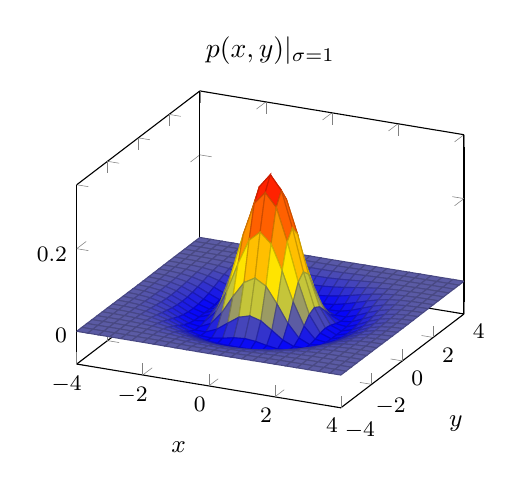
\begin{tikzpicture}
    \begin{axis}[
        title={$p(x,y)|_{\sigma=1}$}, 
        xlabel=$x$, ylabel=$y$,
    	small,
    ]
    \addplot3[
    	surf,
    	domain=-4:4,
    	domain y=-4:4,
    ] 
    	{1/(3.14)*(1-((x^2+y^2)/1)/2)*exp(-(x^2+y^2)/2)};
    \end{axis}
    \end{tikzpicture}
\end{center}

\begin{figure}[H]
    \centering
    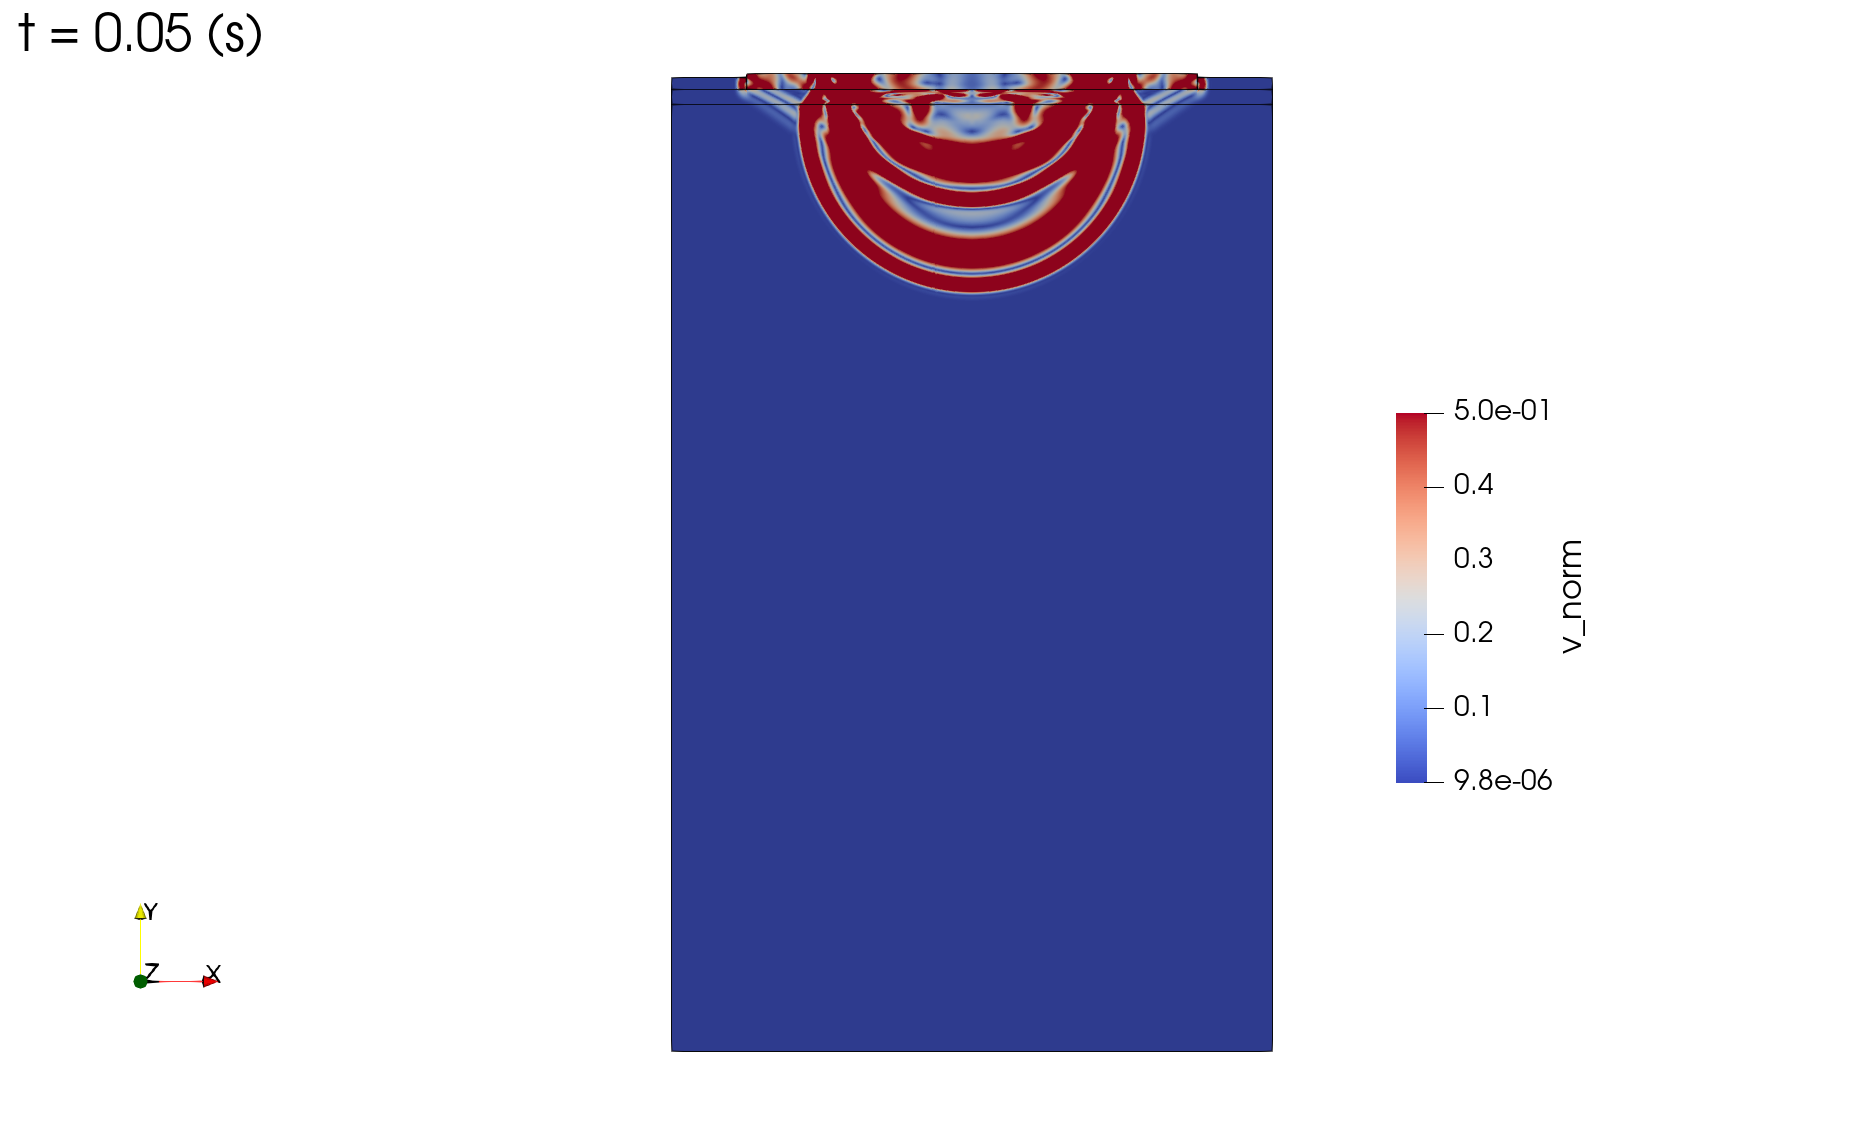
\includegraphics[trim={20cm 1cm 20cm 3cm},clip,width=0.32\textwidth]
    {images/gas_field/0.05.png}
    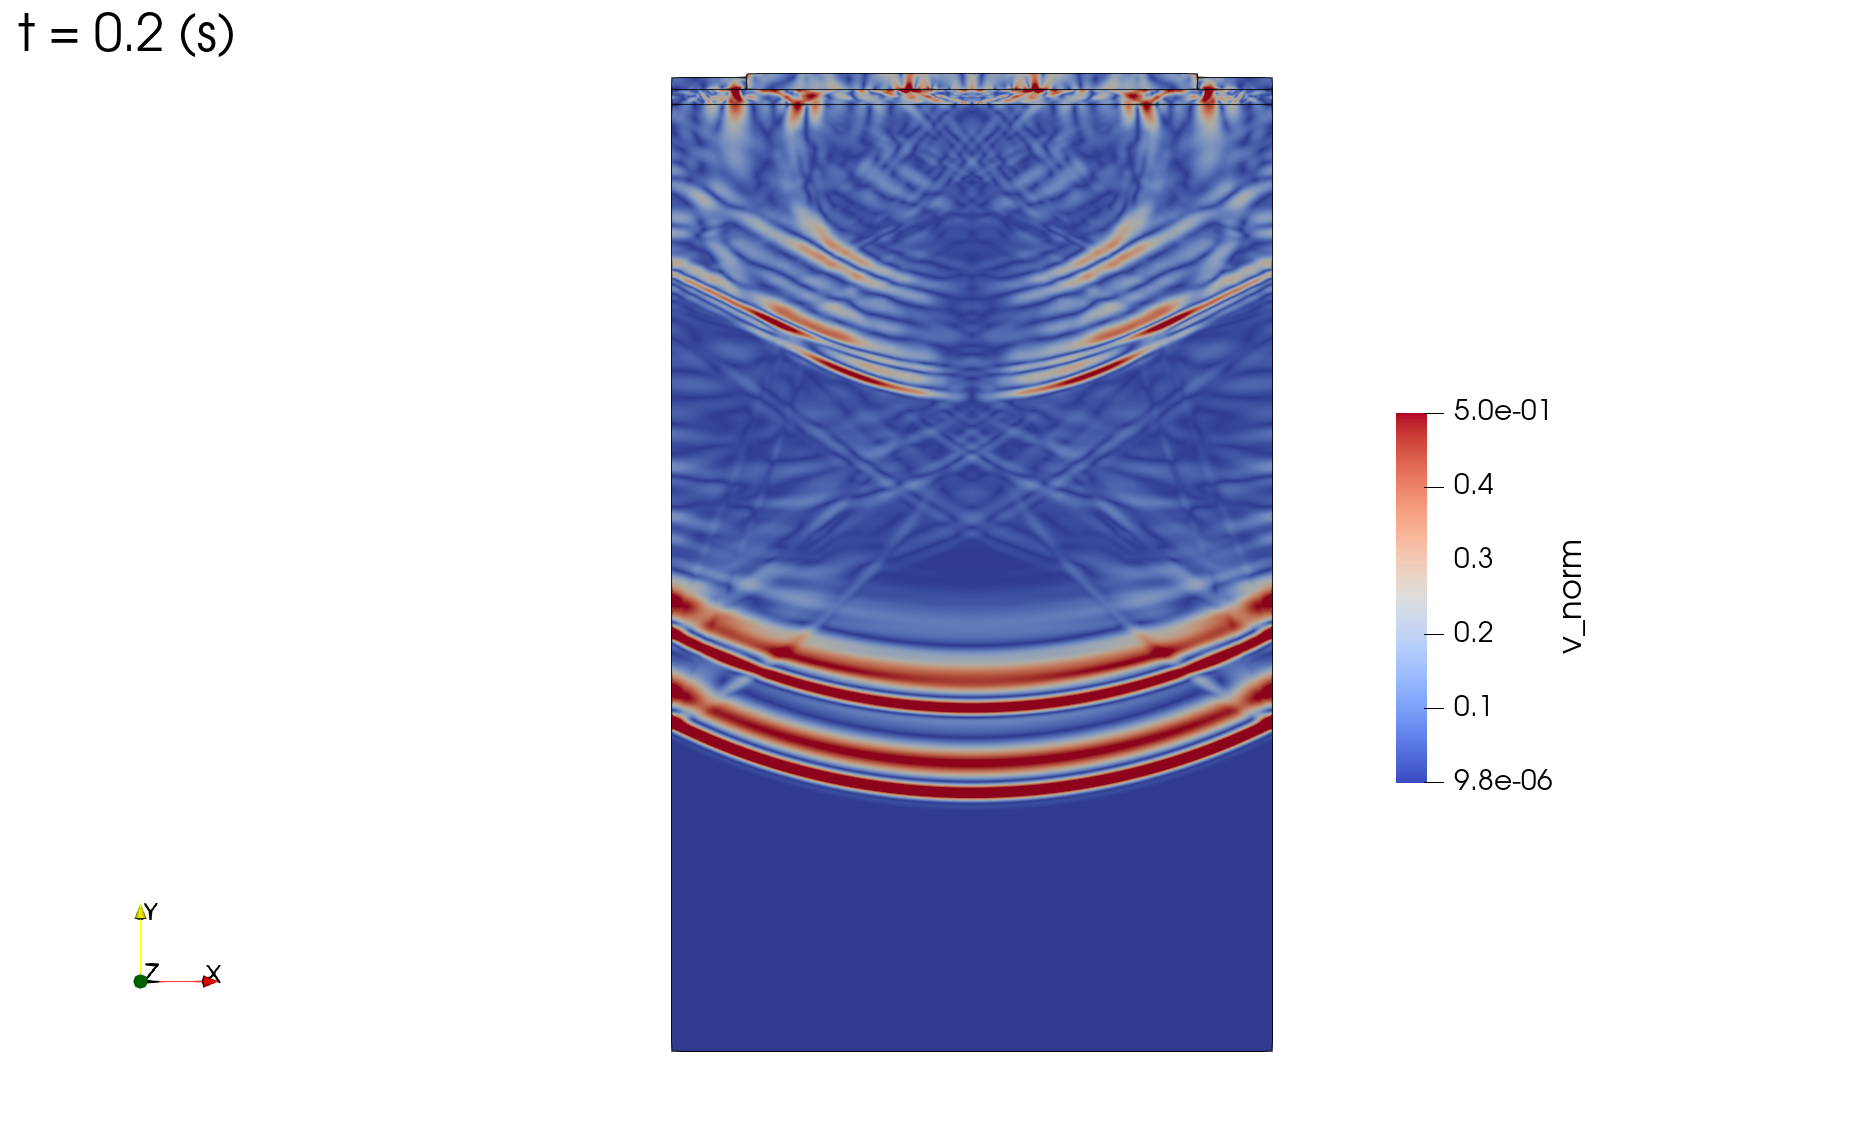
\includegraphics[trim={20cm 1cm 20cm 3cm},clip,width=0.32\textwidth]
    {images/gas_field/0.20.png}
    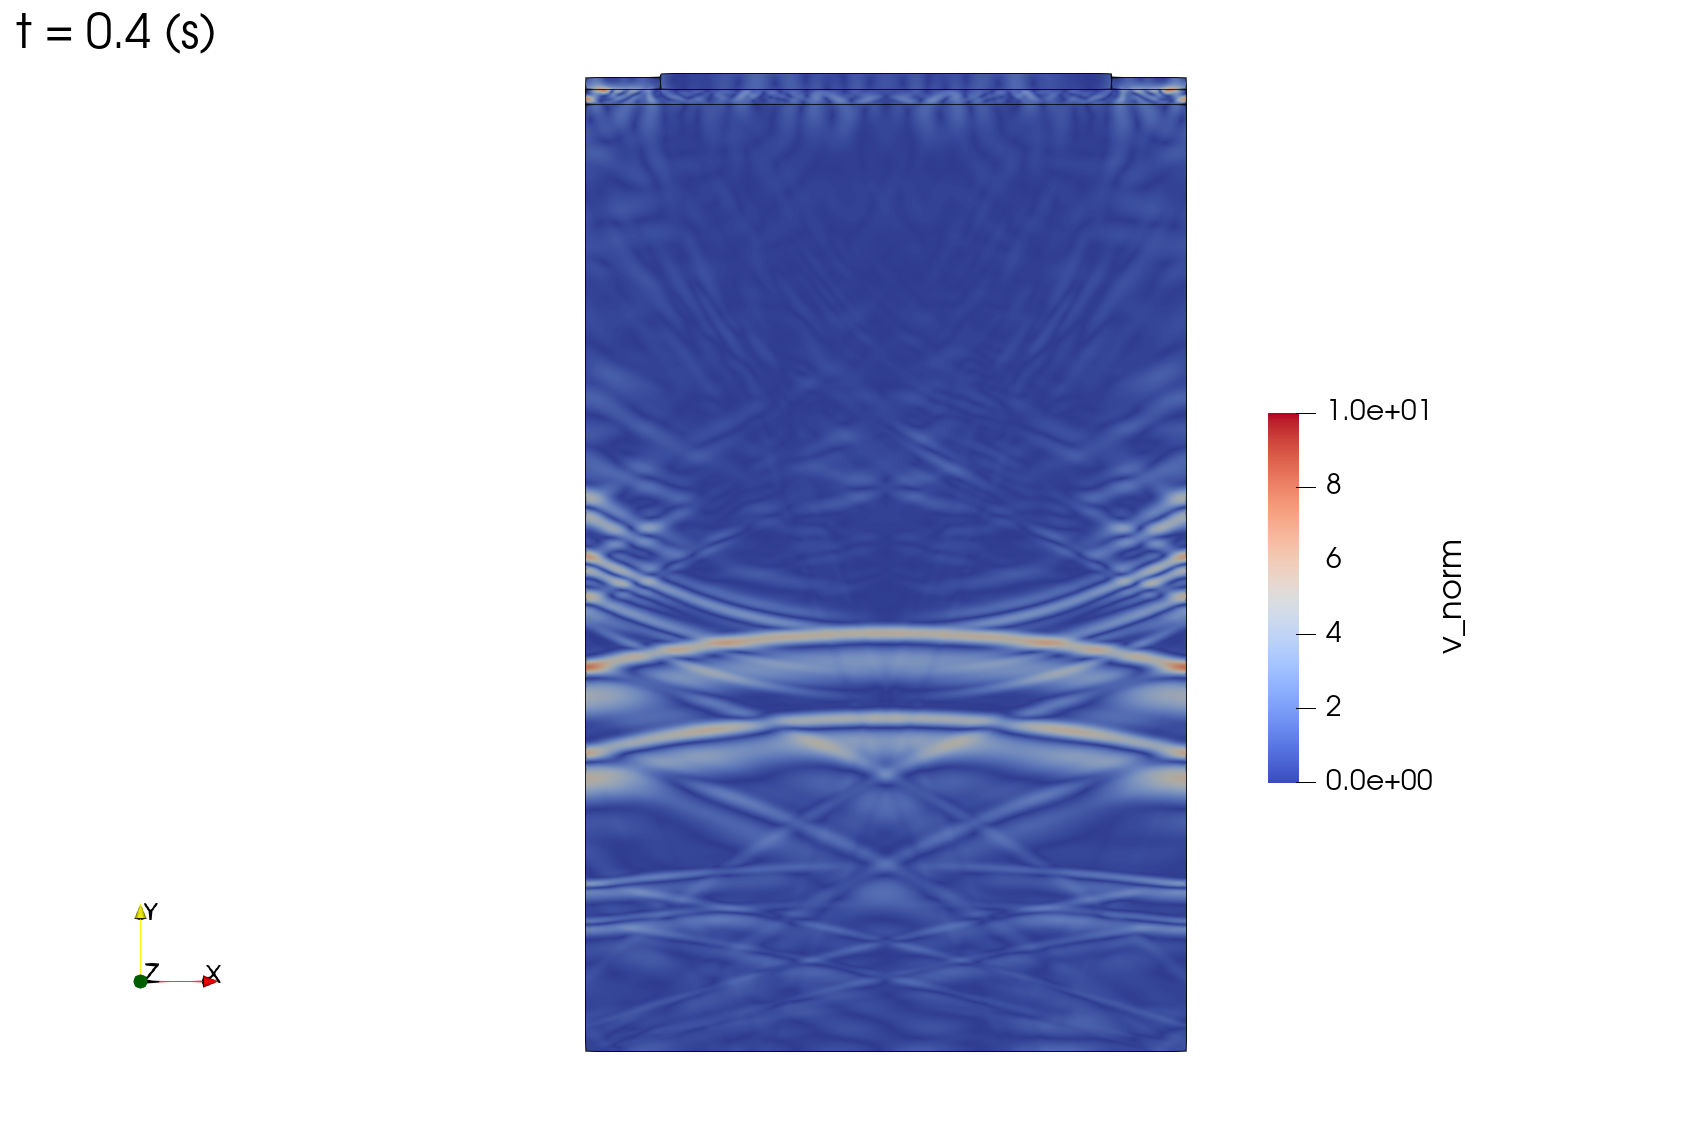
\includegraphics[trim={20cm 1cm 20cm 3cm},clip,width=0.32\textwidth]
    {images/gas_field/0.40.png}\\
    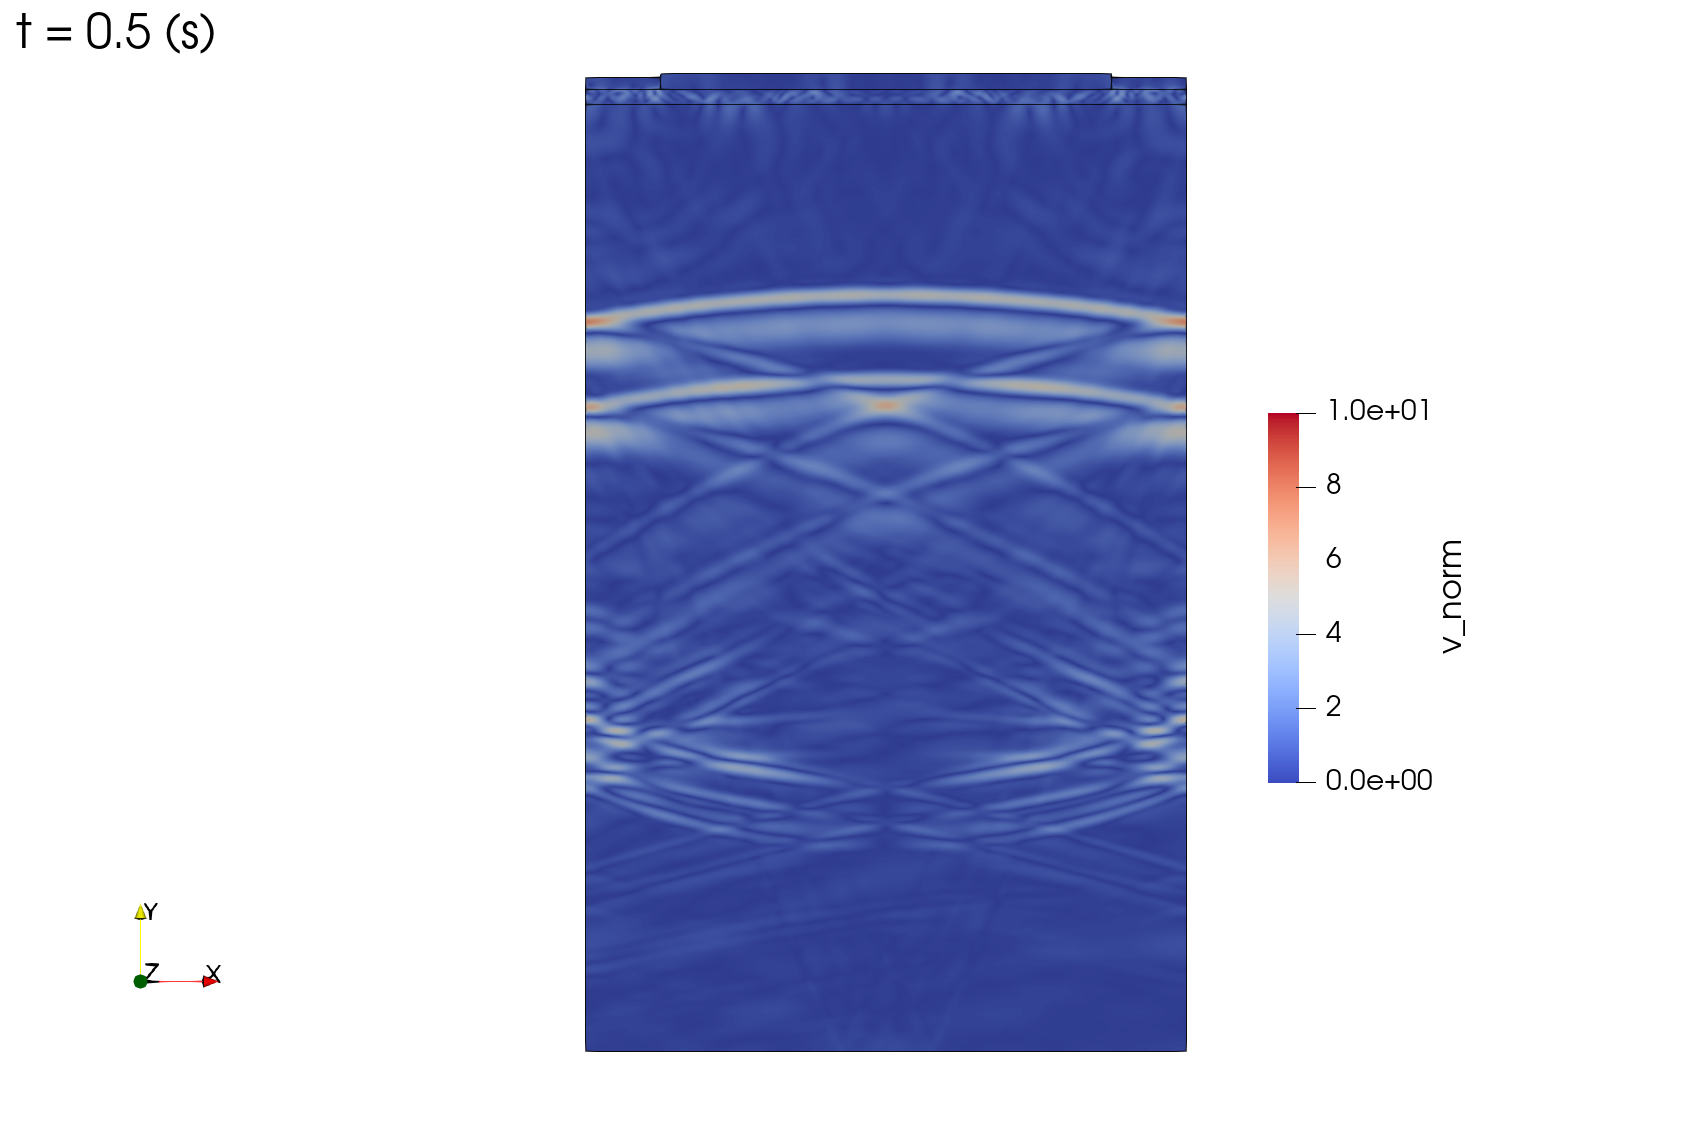
\includegraphics[trim={20cm 1cm 20cm 3cm},clip,width=0.32\textwidth]
    {images/gas_field/0.50.png}
    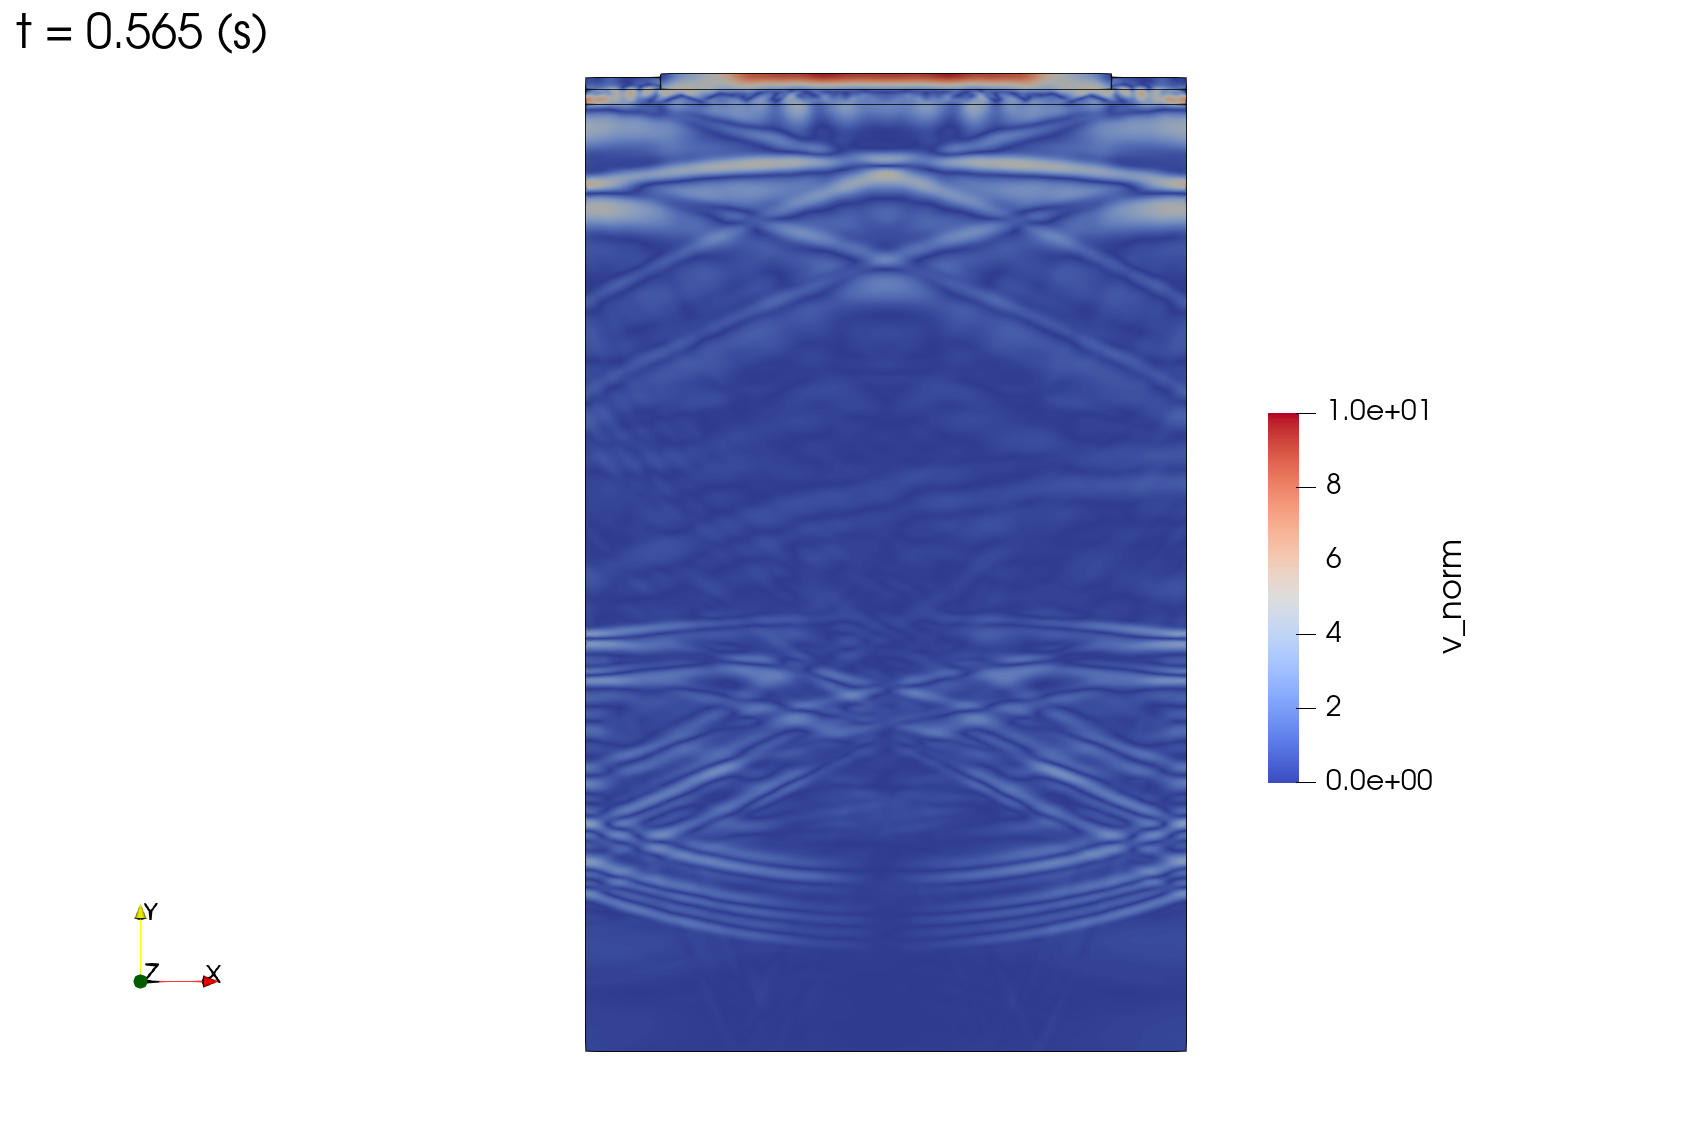
\includegraphics[trim={20cm 1cm 20cm 3cm},clip,width=0.32\textwidth]
    {images/gas_field/0.565.png}
    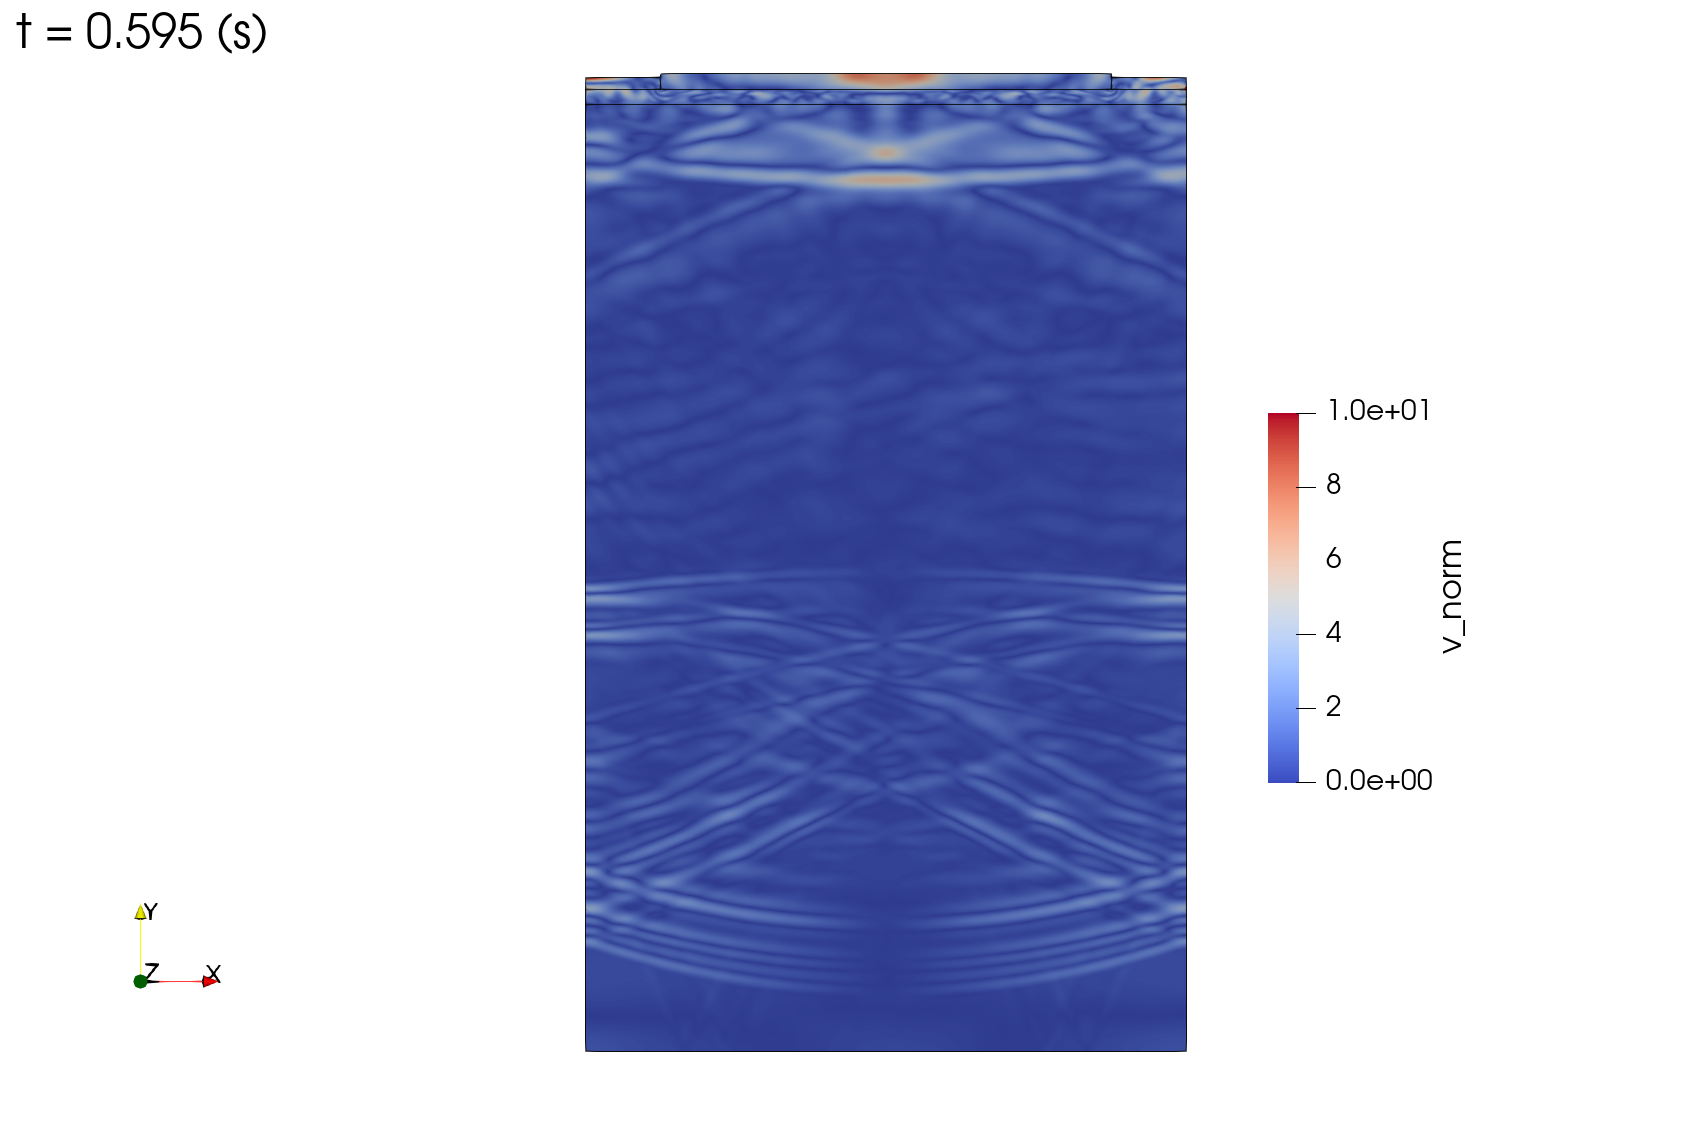
\includegraphics[trim={20cm 1cm 20cm 3cm},clip,width=0.32\textwidth]
    {images/gas_field/0.595.png}
    \caption{Волновая картина.}
    \label{fig:wave_image}
\end{figure}

\subsection{Моделирование статической нагрузке (задача о штампе)}
